% Generated by eval/scripts/write_belebele_profiles.py; released scores unchanged.
\definecolor{belebeleif}{RGB}{35,103,159}
\definecolor{belebelecons}{RGB}{202,86,42}
\definecolor{belebelespec}{RGB}{38,132,109}
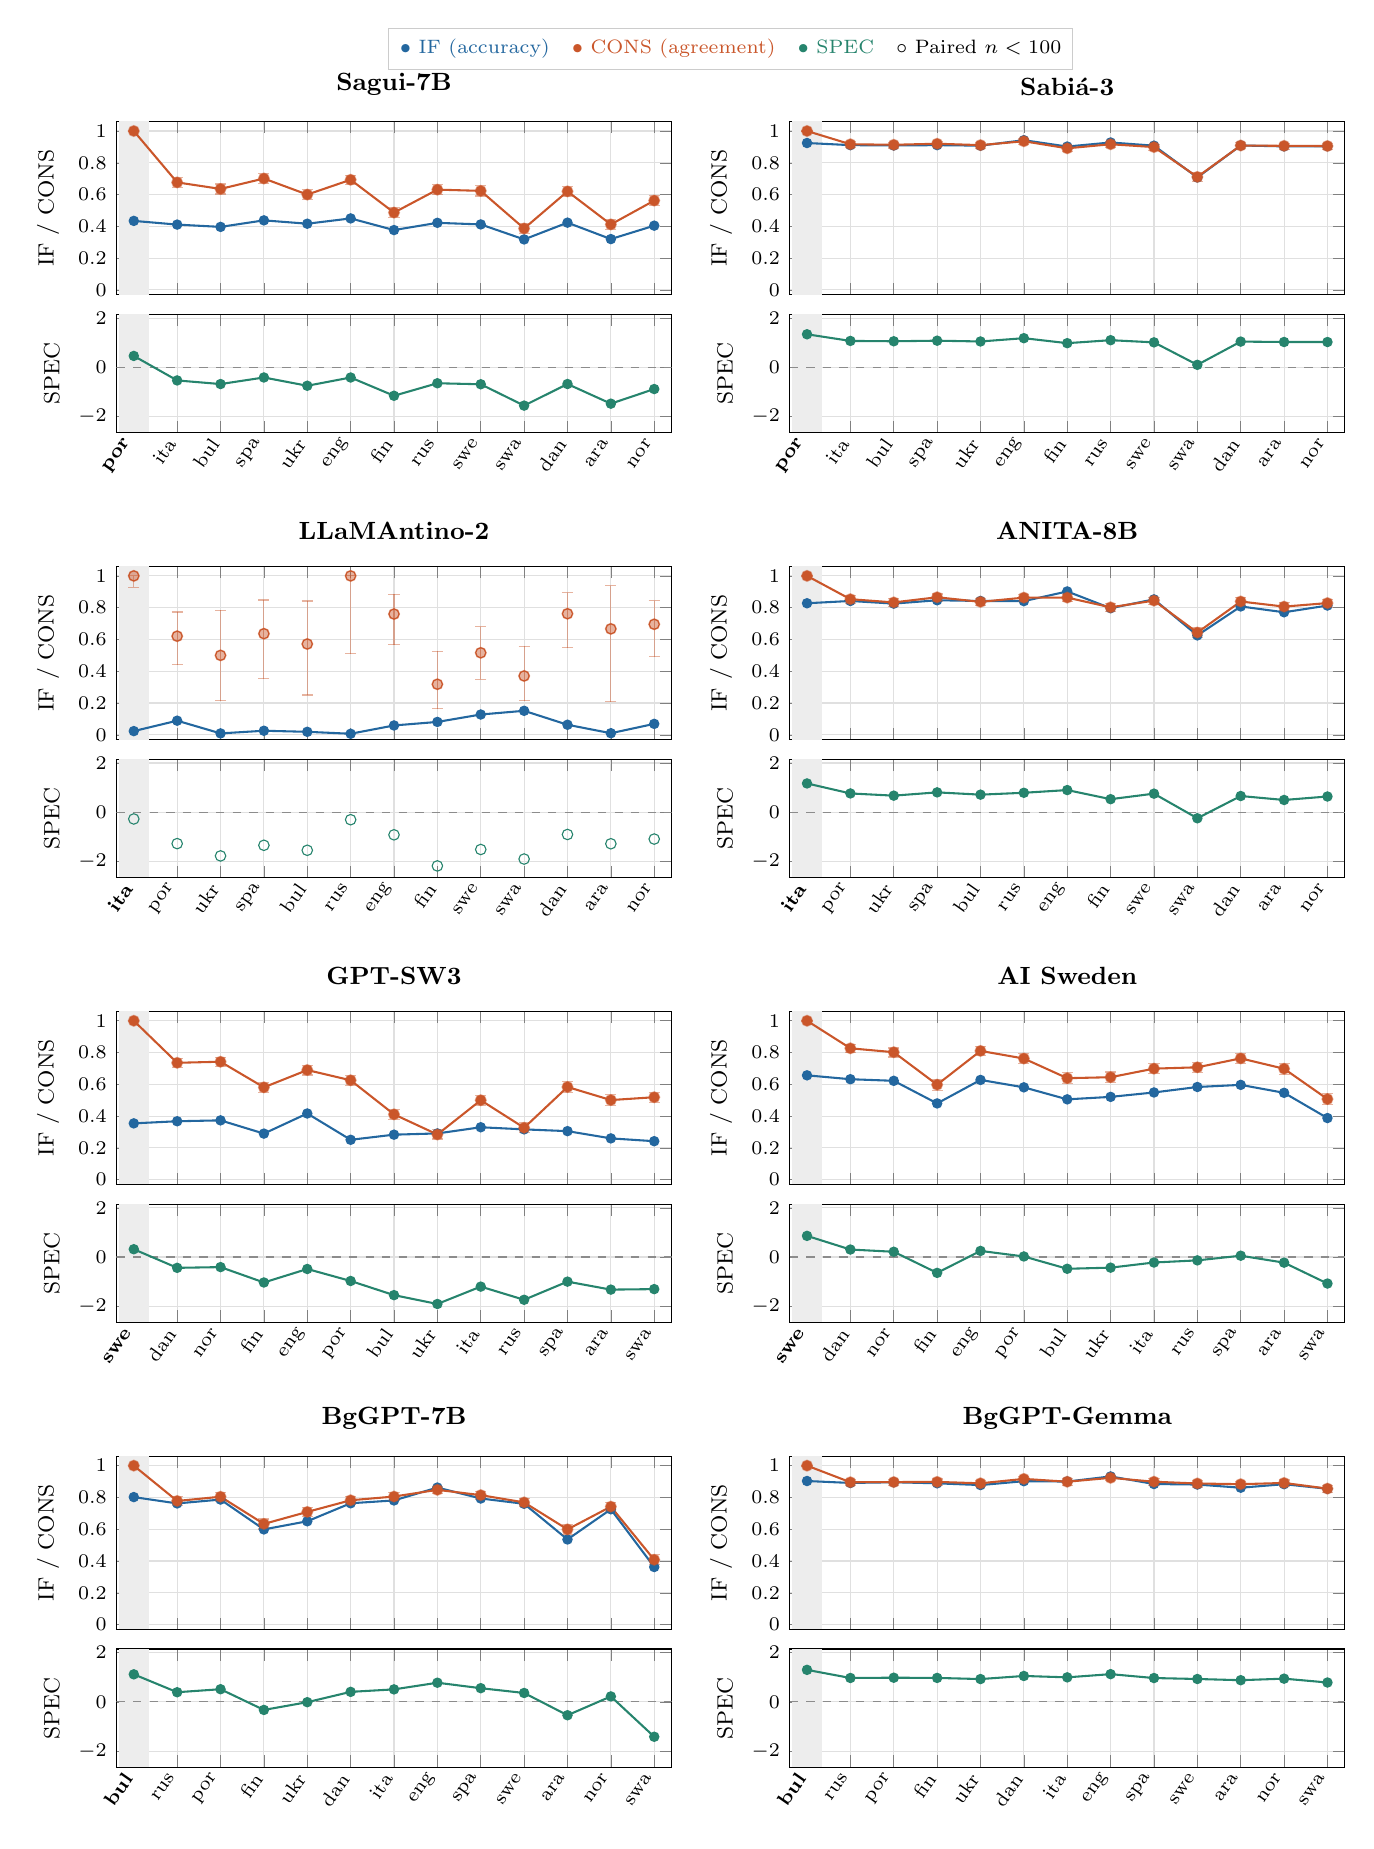
\begin{tikzpicture}
\pgfplotsset{belebeleaxis/.style={width=7.05cm,scale only axis,xmin=-.4,xmax=12.4,
axis lines=box,grid=major,grid style={black!12},
tick label style={font=\scriptsize},label style={font=\footnotesize},
title style={font=\bfseries\small},unbounded coords=jump,
clip=true,xtick={0,...,12}}}
\node[anchor=south,draw=black!20,fill=white,inner sep=4pt,font=\scriptsize] at (7.8,.65) {\textcolor{belebeleif}{$\bullet$ IF (accuracy)}\quad
\textcolor{belebelecons}{$\bullet$ CONS (agreement)}\quad
\textcolor{belebelespec}{$\bullet$ SPEC}\quad $\circ$ Paired $n<100$};
\begin{axis}[belebeleaxis,height=2.2cm,at={(0.00cm,0.00cm)},anchor=north west,
title={Sagui-7B},
ymin=-.03,ymax=1.06,ytick={0,.2,.4,.6,.8,1},xticklabels=\empty,ylabel={IF / CONS}]
\path[fill=black!7] (axis cs:-.35,-.03) rectangle (axis cs:.35,1.06);
\addplot[color=belebeleif,mark=*,mark size=1.5pt,line width=.75pt] coordinates {(0,0.434444) (1,0.411111) (2,0.396667) (3,0.437778) (4,0.416667) (5,0.450000) (6,0.376667) (7,0.422222) (8,0.412222) (9,0.317778) (10,0.423333) (11,0.320000) (12,0.404444)};
\addplot[color=belebelecons,mark=*,mark size=1.5pt,line width=.75pt] coordinates {(0,1.000000) (1,0.676667) (2,0.635556) (3,0.701111) (4,0.600000) (5,0.693333) (6,0.486667) (7,0.631111) (8,0.623333) (9,0.386667) (10,0.620000) (11,0.412222) (12,0.562222)};
\addplot[color=belebelecons,opacity=.45,only marks,mark=none,error bars/.cd,y dir=both,y explicit] coordinates {(0,1.000000) += (0,0.000000) -= (0,0.004250) (1,0.676667) += (0,0.029752) -= (0,0.031254) (2,0.635556) += (0,0.030805) -= (0,0.031957) (3,0.701111) += (0,0.029001) -= (0,0.030711) (4,0.600000) += (0,0.031516) -= (0,0.032366) (5,0.693333) += (0,0.029251) -= (0,0.030894) (6,0.486667) += (0,0.032642) -= (0,0.032528) (7,0.631111) += (0,0.030904) -= (0,0.032018) (8,0.623333) += (0,0.031070) -= (0,0.032118) (9,0.386667) += (0,0.032234) -= (0,0.031270) (10,0.620000) += (0,0.031138) -= (0,0.032158) (11,0.412222) += (0,0.032466) -= (0,0.031719) (12,0.562222) += (0,0.032080) -= (0,0.032609)};
\addplot[color=belebelecons,only marks,mark=o,mark options={fill=white},mark size=1.8pt] coordinates {            };
\end{axis}
\begin{axis}[belebeleaxis,height=1.5cm,at={(0.00cm,-2.45cm)},anchor=north west,
ymin=-2.65,ymax=2.15,ytick={-2,0,2},xticklabels={\textbf{por},ita,bul,spa,ukr,eng,fin,rus,swe,swa,dan,ara,nor},x tick label style={rotate=55,anchor=east,font=\scriptsize},ylabel={SPEC}]
\path[fill=black!7] (axis cs:-.35,-2.65) rectangle (axis cs:.35,2.15);
\addplot[black!45,dashed,mark=none] coordinates {(-.4,0) (12.4,0)};
\addplot[color=belebelespec,mark=*,mark size=1.5pt,line width=.75pt] coordinates {(0,0.461719) (1,-0.534344) (2,-0.681593) (3,-0.414341) (4,-0.750621) (5,-0.415355) (6,-1.156874) (7,-0.648837) (8,-0.689740) (9,-1.557684) (10,-0.679633) (11,-1.478279) (12,-0.884044)};
\addplot[color=belebelespec,only marks,mark=o,mark options={fill=white},mark size=1.9pt] coordinates {            };
\end{axis}
\begin{axis}[belebeleaxis,height=2.2cm,at={(8.55cm,0.00cm)},anchor=north west,
title={Sabi\'a-3},
ymin=-.03,ymax=1.06,ytick={0,.2,.4,.6,.8,1},xticklabels=\empty,ylabel={IF / CONS}]
\path[fill=black!7] (axis cs:-.35,-.03) rectangle (axis cs:.35,1.06);
\addplot[color=belebeleif,mark=*,mark size=1.5pt,line width=.75pt] coordinates {(0,0.924444) (1,0.911111) (2,0.908889) (3,0.911111) (4,0.907778) (5,0.942222) (6,0.902222) (7,0.927778) (8,0.907778) (9,0.707778) (10,0.908889) (11,0.903333) (12,0.904444)};
\addplot[color=belebelecons,mark=*,mark size=1.5pt,line width=.75pt] coordinates {(0,1.000000) (1,0.916667) (2,0.913333) (3,0.919911) (4,0.911111) (5,0.935556) (6,0.891111) (7,0.916667) (8,0.898889) (9,0.711111) (10,0.908788) (11,0.906667) (12,0.905556)};
\addplot[color=belebelecons,opacity=.45,only marks,mark=none,error bars/.cd,y dir=both,y explicit] coordinates {(0,1.000000) += (0,0.000000) -= (0,0.004250) (1,0.916667) += (0,0.016334) -= (0,0.019876) (2,0.913333) += (0,0.016669) -= (0,0.020182) (3,0.919911) += (0,0.016008) -= (0,0.019582) (4,0.911111) += (0,0.016888) -= (0,0.020382) (5,0.935556) += (0,0.014263) -= (0,0.017966) (6,0.891111) += (0,0.018713) -= (0,0.022038) (7,0.916667) += (0,0.016334) -= (0,0.019876) (8,0.898889) += (0,0.018032) -= (0,0.021422) (9,0.711111) += (0,0.028665) -= (0,0.030459) (10,0.908788) += (0,0.017121) -= (0,0.020600) (11,0.906667) += (0,0.017315) -= (0,0.020772) (12,0.905556) += (0,0.017420) -= (0,0.020867)};
\addplot[color=belebelecons,only marks,mark=o,mark options={fill=white},mark size=1.8pt] coordinates {            };
\end{axis}
\begin{axis}[belebeleaxis,height=1.5cm,at={(8.55cm,-2.45cm)},anchor=north west,
ymin=-2.65,ymax=2.15,ytick={-2,0,2},xticklabels={\textbf{por},ita,bul,spa,ukr,eng,fin,rus,swe,swa,dan,ara,nor},x tick label style={rotate=55,anchor=east,font=\scriptsize},ylabel={SPEC}]
\path[fill=black!7] (axis cs:-.35,-2.65) rectangle (axis cs:.35,2.15);
\addplot[black!45,dashed,mark=none] coordinates {(-.4,0) (12.4,0)};
\addplot[color=belebelespec,mark=*,mark size=1.5pt,line width=.75pt] coordinates {(0,1.341249) (1,1.071393) (2,1.057568) (3,1.080968) (4,1.049015) (5,1.182979) (6,0.980022) (7,1.101309) (8,1.012947) (9,0.099809) (10,1.044153) (11,1.027922) (12,1.026637)};
\addplot[color=belebelespec,only marks,mark=o,mark options={fill=white},mark size=1.9pt] coordinates {            };
\end{axis}
\begin{axis}[belebeleaxis,height=2.2cm,at={(0.00cm,-5.65cm)},anchor=north west,
title={LLaMAntino-2},
ymin=-.03,ymax=1.06,ytick={0,.2,.4,.6,.8,1},xticklabels=\empty,ylabel={IF / CONS}]
\path[fill=black!7] (axis cs:-.35,-.03) rectangle (axis cs:.35,1.06);
\addplot[color=belebeleif,mark=*,mark size=1.5pt,line width=.75pt] coordinates {(0,0.023333) (1,0.088889) (2,0.008889) (3,0.025556) (4,0.018889) (5,0.006667) (6,0.058889) (7,0.081111) (8,0.127778) (9,0.151111) (10,0.063333) (11,0.010000) (12,0.068889)};
\addplot[color=belebelecons,mark=*,mark size=1.5pt,line width=.75pt] coordinates {(0,nan) (1,nan) (2,nan) (3,nan) (4,nan) (5,nan) (6,nan) (7,nan) (8,nan) (9,nan) (10,nan) (11,nan) (12,nan)};
\addplot[color=belebelecons,opacity=.45,only marks,mark=none,error bars/.cd,y dir=both,y explicit] coordinates {(0,1.000000) += (0,0.000000) -= (0,0.071348) (1,0.620690) += (0,0.152430) -= (0,0.180664) (2,0.500000) += (0,0.284784) -= (0,0.284784) (3,0.636364) += (0,0.211972) -= (0,0.282562) (4,0.571429) += (0,0.270352) -= (0,0.320970) (5,1.000000) += (0,0.000000) -= (0,0.489891) (6,0.760000) += (0,0.125037) -= (0,0.194297) (7,0.318182) += (0,0.208632) -= (0,0.154576) (8,0.516129) += (0,0.164168) -= (0,0.167725) (9,0.370370) += (0,0.187337) -= (0,0.155045) (10,0.761905) += (0,0.131815) -= (0,0.212816) (11,0.666667) += (0,0.271841) -= (0,0.459007) (12,0.695652) += (0,0.148308) -= (0,0.204310)};
\addplot[color=belebelecons,only marks,mark=o,mark options={fill=white},mark size=1.8pt] coordinates {(0,1.000000) (1,0.620690) (2,0.500000) (3,0.636364) (4,0.571429) (5,1.000000) (6,0.760000) (7,0.318182) (8,0.516129) (9,0.370370) (10,0.761905) (11,0.666667) (12,0.695652)};
\end{axis}
\begin{axis}[belebeleaxis,height=1.5cm,at={(0.00cm,-8.10cm)},anchor=north west,
ymin=-2.65,ymax=2.15,ytick={-2,0,2},xticklabels={\textbf{ita},por,ukr,spa,bul,rus,eng,fin,swe,swa,dan,ara,nor},x tick label style={rotate=55,anchor=east,font=\scriptsize},ylabel={SPEC}]
\path[fill=black!7] (axis cs:-.35,-2.65) rectangle (axis cs:.35,2.15);
\addplot[black!45,dashed,mark=none] coordinates {(-.4,0) (12.4,0)};
\addplot[color=belebelespec,mark=*,mark size=1.5pt,line width=.75pt] coordinates {(0,nan) (1,nan) (2,nan) (3,nan) (4,nan) (5,nan) (6,nan) (7,nan) (8,nan) (9,nan) (10,nan) (11,nan) (12,nan)};
\addplot[color=belebelespec,only marks,mark=o,mark options={fill=white},mark size=1.9pt] coordinates {(0,-0.276208) (1,-1.277911) (2,-1.777672) (3,-1.345337) (4,-1.548931) (5,-0.306124) (6,-0.920645) (7,-2.184595) (8,-1.516673) (9,-1.904936) (10,-0.907046) (11,-1.283832) (12,-1.092590)};
\end{axis}
\begin{axis}[belebeleaxis,height=2.2cm,at={(8.55cm,-5.65cm)},anchor=north west,
title={ANITA-8B},
ymin=-.03,ymax=1.06,ytick={0,.2,.4,.6,.8,1},xticklabels=\empty,ylabel={IF / CONS}]
\path[fill=black!7] (axis cs:-.35,-.03) rectangle (axis cs:.35,1.06);
\addplot[color=belebeleif,mark=*,mark size=1.5pt,line width=.75pt] coordinates {(0,0.827778) (1,0.842222) (2,0.825556) (3,0.846667) (4,0.842222) (5,0.841111) (6,0.902222) (7,0.796667) (8,0.852222) (9,0.625556) (10,0.807778) (11,0.771111) (12,0.813333)};
\addplot[color=belebelecons,mark=*,mark size=1.5pt,line width=.75pt] coordinates {(0,1.000000) (1,0.853333) (2,0.833148) (3,0.865556) (4,0.836667) (5,0.863181) (6,0.863333) (7,0.802222) (8,0.844444) (9,0.643333) (10,0.838889) (11,0.806667) (12,0.828889)};
\addplot[color=belebelecons,opacity=.45,only marks,mark=none,error bars/.cd,y dir=both,y explicit] coordinates {(0,1.000000) += (0,0.000000) -= (0,0.004250) (1,0.853333) += (0,0.021611) -= (0,0.024614) (2,0.833148) += (0,0.022944) -= (0,0.025779) (3,0.865556) += (0,0.020740) -= (0,0.023847) (4,0.836667) += (0,0.022711) -= (0,0.025573) (5,0.863181) += (0,0.020924) -= (0,0.024015) (6,0.863333) += (0,0.020902) -= (0,0.023991) (7,0.802222) += (0,0.024715) -= (0,0.027284) (8,0.844444) += (0,0.022210) -= (0,0.025137) (9,0.643333) += (0,0.030625) -= (0,0.031844) (10,0.838889) += (0,0.022570) -= (0,0.025451) (11,0.806667) += (0,0.024475) -= (0,0.027082) (12,0.828889) += (0,0.023194) -= (0,0.025990)};
\addplot[color=belebelecons,only marks,mark=o,mark options={fill=white},mark size=1.8pt] coordinates {            };
\end{axis}
\begin{axis}[belebeleaxis,height=1.5cm,at={(8.55cm,-8.10cm)},anchor=north west,
ymin=-2.65,ymax=2.15,ytick={-2,0,2},xticklabels={\textbf{ita},por,ukr,spa,bul,rus,eng,fin,swe,swa,dan,ara,nor},x tick label style={rotate=55,anchor=east,font=\scriptsize},ylabel={SPEC}]
\path[fill=black!7] (axis cs:-.35,-2.65) rectangle (axis cs:.35,2.15);
\addplot[black!45,dashed,mark=none] coordinates {(-.4,0) (12.4,0)};
\addplot[color=belebelespec,mark=*,mark size=1.5pt,line width=.75pt] coordinates {(0,1.167736) (1,0.760839) (2,0.671355) (3,0.804886) (4,0.711655) (5,0.787907) (6,0.898047) (7,0.528236) (8,0.752557) (9,-0.247794) (10,0.656386) (11,0.495481) (12,0.636848)};
\addplot[color=belebelespec,only marks,mark=o,mark options={fill=white},mark size=1.9pt] coordinates {            };
\end{axis}
\begin{axis}[belebeleaxis,height=2.2cm,at={(0.00cm,-11.30cm)},anchor=north west,
title={GPT-SW3},
ymin=-.03,ymax=1.06,ytick={0,.2,.4,.6,.8,1},xticklabels=\empty,ylabel={IF / CONS}]
\path[fill=black!7] (axis cs:-.35,-.03) rectangle (axis cs:.35,1.06);
\addplot[color=belebeleif,mark=*,mark size=1.5pt,line width=.75pt] coordinates {(0,0.354444) (1,0.367778) (2,0.373333) (3,0.290000) (4,0.416667) (5,0.251111) (6,0.283333) (7,0.291111) (8,0.330000) (9,0.316667) (10,0.305556) (11,0.260000) (12,0.242222)};
\addplot[color=belebelecons,mark=*,mark size=1.5pt,line width=.75pt] coordinates {(0,1.000000) (1,0.735556) (2,0.742222) (3,0.581111) (4,0.690000) (5,0.625556) (6,0.411111) (7,0.284444) (8,0.500000) (9,0.326667) (10,0.583333) (11,0.501111) (12,0.518889)};
\addplot[color=belebelecons,opacity=.45,only marks,mark=none,error bars/.cd,y dir=both,y explicit] coordinates {(0,1.000000) += (0,0.000000) -= (0,0.004250) (1,0.735556) += (0,0.027769) -= (0,0.029771) (2,0.742222) += (0,0.027505) -= (0,0.029564) (3,0.581111) += (0,0.031822) -= (0,0.032511) (4,0.690000) += (0,0.029355) -= (0,0.030970) (5,0.625556) += (0,0.031023) -= (0,0.032090) (6,0.411111) += (0,0.032457) -= (0,0.031702) (7,0.284444) += (0,0.030342) -= (0,0.028510) (8,0.500000) += (0,0.032597) -= (0,0.032597) (9,0.326667) += (0,0.031321) -= (0,0.029847) (10,0.583333) += (0,0.031788) -= (0,0.032497) (11,0.501111) += (0,0.032592) -= (0,0.032601) (12,0.518889) += (0,0.032493) -= (0,0.032654)};
\addplot[color=belebelecons,only marks,mark=o,mark options={fill=white},mark size=1.8pt] coordinates {            };
\end{axis}
\begin{axis}[belebeleaxis,height=1.5cm,at={(0.00cm,-13.75cm)},anchor=north west,
ymin=-2.65,ymax=2.15,ytick={-2,0,2},xticklabels={\textbf{swe},dan,nor,fin,eng,por,bul,ukr,ita,rus,spa,ara,swa},x tick label style={rotate=55,anchor=east,font=\scriptsize},ylabel={SPEC}]
\path[fill=black!7] (axis cs:-.35,-2.65) rectangle (axis cs:.35,2.15);
\addplot[black!45,dashed,mark=none] coordinates {(-.4,0) (12.4,0)};
\addplot[color=belebelespec,mark=*,mark size=1.5pt,line width=.75pt] coordinates {(0,0.318123) (1,-0.438340) (2,-0.408694) (3,-1.033724) (4,-0.485024) (5,-0.972369) (6,-1.547373) (7,-1.907215) (8,-1.201291) (9,-1.736743) (10,-0.999245) (11,-1.323659) (12,-1.303106)};
\addplot[color=belebelespec,only marks,mark=o,mark options={fill=white},mark size=1.9pt] coordinates {            };
\end{axis}
\begin{axis}[belebeleaxis,height=2.2cm,at={(8.55cm,-11.30cm)},anchor=north west,
title={AI Sweden},
ymin=-.03,ymax=1.06,ytick={0,.2,.4,.6,.8,1},xticklabels=\empty,ylabel={IF / CONS}]
\path[fill=black!7] (axis cs:-.35,-.03) rectangle (axis cs:.35,1.06);
\addplot[color=belebeleif,mark=*,mark size=1.5pt,line width=.75pt] coordinates {(0,0.656667) (1,0.632222) (2,0.622222) (3,0.480000) (4,0.627778) (5,0.581111) (6,0.505556) (7,0.521111) (8,0.548889) (9,0.583333) (10,0.596667) (11,0.546667) (12,0.387778)};
\addplot[color=belebelecons,mark=*,mark size=1.5pt,line width=.75pt] coordinates {(0,1.000000) (1,0.826772) (2,0.802125) (3,0.597938) (4,0.810414) (5,0.762467) (6,0.638710) (7,0.644872) (8,0.698827) (9,0.707161) (10,0.763399) (11,0.698138) (12,0.507285)};
\addplot[color=belebelecons,opacity=.45,only marks,mark=none,error bars/.cd,y dir=both,y explicit] coordinates {(0,1.000000) += (0,0.000000) -= (0,0.004755) (1,0.826772) += (0,0.025214) -= (0,0.028492) (2,0.802125) += (0,0.026891) -= (0,0.029958) (3,0.597938) += (0,0.033934) -= (0,0.034899) (4,0.810414) += (0,0.026461) -= (0,0.029628) (5,0.762467) += (0,0.028853) -= (0,0.031486) (6,0.638710) += (0,0.033060) -= (0,0.034428) (7,0.644872) += (0,0.032799) -= (0,0.034219) (8,0.698827) += (0,0.031410) -= (0,0.033392) (9,0.707161) += (0,0.030820) -= (0,0.032845) (10,0.763399) += (0,0.028754) -= (0,0.031386) (11,0.698138) += (0,0.031736) -= (0,0.033750) (12,0.507285) += (0,0.035534) -= (0,0.035608)};
\addplot[color=belebelecons,only marks,mark=o,mark options={fill=white},mark size=1.8pt] coordinates {            };
\end{axis}
\begin{axis}[belebeleaxis,height=1.5cm,at={(8.55cm,-13.75cm)},anchor=north west,
ymin=-2.65,ymax=2.15,ytick={-2,0,2},xticklabels={\textbf{swe},dan,nor,fin,eng,por,bul,ukr,ita,rus,spa,ara,swa},x tick label style={rotate=55,anchor=east,font=\scriptsize},ylabel={SPEC}]
\path[fill=black!7] (axis cs:-.35,-2.65) rectangle (axis cs:.35,2.15);
\addplot[black!45,dashed,mark=none] coordinates {(-.4,0) (12.4,0)};
\addplot[color=belebelespec,mark=*,mark size=1.5pt,line width=.75pt] coordinates {(0,0.860599) (1,0.305513) (2,0.214828) (3,-0.643025) (4,0.249262) (5,0.024003) (6,-0.476834) (7,-0.430727) (8,-0.221643) (9,-0.135220) (10,0.054674) (11,-0.227663) (12,-1.076084)};
\addplot[color=belebelespec,only marks,mark=o,mark options={fill=white},mark size=1.9pt] coordinates {            };
\end{axis}
\begin{axis}[belebeleaxis,height=2.2cm,at={(0.00cm,-16.95cm)},anchor=north west,
title={BgGPT-7B},
ymin=-.03,ymax=1.06,ytick={0,.2,.4,.6,.8,1},xticklabels=\empty,ylabel={IF / CONS}]
\path[fill=black!7] (axis cs:-.35,-.03) rectangle (axis cs:.35,1.06);
\addplot[color=belebeleif,mark=*,mark size=1.5pt,line width=.75pt] coordinates {(0,0.802222) (1,0.762222) (2,0.786667) (3,0.598889) (4,0.650000) (5,0.763333) (6,0.781111) (7,0.862222) (8,0.793333) (9,0.760000) (10,0.535556) (11,0.725556) (12,0.362222)};
\addplot[color=belebelecons,mark=*,mark size=1.5pt,line width=.75pt] coordinates {(0,1.000000) (1,0.777778) (2,0.804444) (3,0.633333) (4,0.708889) (5,0.782222) (6,0.805556) (7,0.847778) (8,0.814444) (9,0.768889) (10,0.598889) (11,0.742222) (12,0.407778)};
\addplot[color=belebelecons,opacity=.45,only marks,mark=none,error bars/.cd,y dir=both,y explicit] coordinates {(0,1.000000) += (0,0.000000) -= (0,0.004250) (1,0.777778) += (0,0.025948) -= (0,0.028310) (2,0.804444) += (0,0.024596) -= (0,0.027184) (3,0.633333) += (0,0.030855) -= (0,0.031988) (4,0.708889) += (0,0.028741) -= (0,0.030517) (5,0.782222) += (0,0.025735) -= (0,0.028134) (6,0.805556) += (0,0.024536) -= (0,0.027133) (7,0.847778) += (0,0.021988) -= (0,0.024944) (8,0.814444) += (0,0.024042) -= (0,0.026715) (9,0.768889) += (0,0.026363) -= (0,0.028648) (10,0.598889) += (0,0.031535) -= (0,0.032376) (11,0.742222) += (0,0.027505) -= (0,0.029564) (12,0.407778) += (0,0.032432) -= (0,0.031648)};
\addplot[color=belebelecons,only marks,mark=o,mark options={fill=white},mark size=1.8pt] coordinates {            };
\end{axis}
\begin{axis}[belebeleaxis,height=1.5cm,at={(0.00cm,-19.40cm)},anchor=north west,
ymin=-2.65,ymax=2.15,ytick={-2,0,2},xticklabels={\textbf{bul},rus,por,fin,ukr,dan,ita,eng,spa,swe,ara,nor,swa},x tick label style={rotate=55,anchor=east,font=\scriptsize},ylabel={SPEC}]
\path[fill=black!7] (axis cs:-.35,-2.65) rectangle (axis cs:.35,2.15);
\addplot[black!45,dashed,mark=none] coordinates {(-.4,0) (12.4,0)};
\addplot[color=belebelespec,mark=*,mark size=1.5pt,line width=.75pt] coordinates {(0,1.121865) (1,0.394273) (2,0.516845) (3,-0.325170) (4,-0.010458) (5,0.409383) (6,0.510152) (7,0.780344) (8,0.558322) (9,0.364052) (10,-0.540499) (11,0.223530) (12,-1.415608)};
\addplot[color=belebelespec,only marks,mark=o,mark options={fill=white},mark size=1.9pt] coordinates {            };
\end{axis}
\begin{axis}[belebeleaxis,height=2.2cm,at={(8.55cm,-16.95cm)},anchor=north west,
title={BgGPT-Gemma},
ymin=-.03,ymax=1.06,ytick={0,.2,.4,.6,.8,1},xticklabels=\empty,ylabel={IF / CONS}]
\path[fill=black!7] (axis cs:-.35,-.03) rectangle (axis cs:.35,1.06);
\addplot[color=belebeleif,mark=*,mark size=1.5pt,line width=.75pt] coordinates {(0,0.903333) (1,0.891111) (2,0.895556) (3,0.888889) (4,0.877778) (5,0.902222) (6,0.900000) (7,0.932222) (8,0.884444) (9,0.881111) (10,0.861111) (11,0.883333) (12,0.854444)};
\addplot[color=belebelecons,mark=*,mark size=1.5pt,line width=.75pt] coordinates {(0,1.000000) (1,0.895556) (2,0.896667) (3,0.897778) (4,0.888889) (5,0.916667) (6,0.898889) (7,0.923333) (8,0.898889) (9,0.887778) (10,0.883333) (11,0.891111) (12,0.855556)};
\addplot[color=belebelecons,opacity=.45,only marks,mark=none,error bars/.cd,y dir=both,y explicit] coordinates {(0,1.000000) += (0,0.000000) -= (0,0.004250) (1,0.895556) += (0,0.018328) -= (0,0.021690) (2,0.896667) += (0,0.018230) -= (0,0.021602) (3,0.897778) += (0,0.018131) -= (0,0.021512) (4,0.888889) += (0,0.018902) -= (0,0.022208) (5,0.916667) += (0,0.016334) -= (0,0.019876) (6,0.898889) += (0,0.018032) -= (0,0.021422) (7,0.923333) += (0,0.015639) -= (0,0.019238) (8,0.898889) += (0,0.018032) -= (0,0.021422) (9,0.887778) += (0,0.018995) -= (0,0.022292) (10,0.883333) += (0,0.019363) -= (0,0.022621) (11,0.891111) += (0,0.018713) -= (0,0.022038) (12,0.855556) += (0,0.021457) -= (0,0.024479)};
\addplot[color=belebelecons,only marks,mark=o,mark options={fill=white},mark size=1.8pt] coordinates {            };
\end{axis}
\begin{axis}[belebeleaxis,height=1.5cm,at={(8.55cm,-19.40cm)},anchor=north west,
ymin=-2.65,ymax=2.15,ytick={-2,0,2},xticklabels={\textbf{bul},rus,por,fin,ukr,dan,ita,eng,spa,swe,ara,nor,swa},x tick label style={rotate=55,anchor=east,font=\scriptsize},ylabel={SPEC}]
\path[fill=black!7] (axis cs:-.35,-2.65) rectangle (axis cs:.35,2.15);
\addplot[black!45,dashed,mark=none] coordinates {(-.4,0) (12.4,0)};
\addplot[color=belebelespec,mark=*,mark size=1.5pt,line width=.75pt] coordinates {(0,1.303355) (1,0.973194) (2,0.984450) (3,0.975763) (4,0.929587) (5,1.055438) (6,0.998986) (7,1.128961) (8,0.971064) (9,0.932291) (10,0.883276) (11,0.946117) (12,0.789336)};
\addplot[color=belebelespec,only marks,mark=o,mark options={fill=white},mark size=1.9pt] coordinates {            };
\end{axis}
\end{tikzpicture}
